\RequirePackage{luatex85}
\documentclass{standalone}

\usepackage{fontspec, unicode-math}
\setsansfont[Scale=MatchLowercase]{TeX Gyre Heros}
\setmathfont{TeX Gyre Termes Math}

\usepackage{pgfplots}
\pgfplotsset{compat=1.14}

\tikzset{
  every picture/.style={font={\sffamily\normalsize}, >=stealth},
  every pin edge/.style={black}}

\begin{document}

  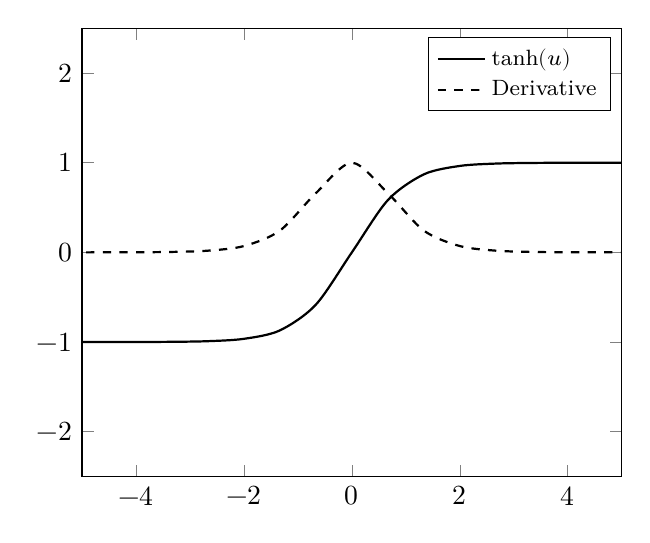
\begin{tikzpicture}
    \begin{axis}[%
        xmax = 5,
        xmin = -5,
        ymax = 2.5,
        ymin = -2.5,
        every axis plot/.style={thick, smooth},
        legend style={font=\footnotesize},
        legend cell align = left]

      \addplot[solid, domain=-8:8] {tanh(\x)};
      \addplot[dashed, domain=-8:8] {1 - pow(tanh(\x), 2))};

      \legend{$\displaystyle \tanh(u)$, Derivative}
    \end{axis}
  \end{tikzpicture}

\end{document}
